%%=============================================================================
%% LaTeX sjabloon voor bachelorproef, HoGent Bedrijf en Organisatie
%% Opleiding Toegepaste Informatica
%%=============================================================================

\documentclass[fleqn,a4paper,12pt]{book}

\usepackage{listings}
\usepackage{xcolor}

%%=============================================================================
%% LaTeX sjabloon voor de bachelorproef, HoGent Bedrijf en Organisatie
%% Opleiding toegepaste informatica
%%
%% Structuur en algemene vormgeving. Meestal hoef je hier niets te wijzigen.
%%
%% Vormgeving gebaseerd op "The Legrand Orange Book", version 2.0 (9/2/15)
%% door Mathias Legrand (legrand.mathias@gmail.com) met aanpassingen door
%% Vel (vel@latextemplates.com). Het oorspronkelijke template is te vinden op
%% http://www.LaTeXTemplates.com
%%
%% Aanpassingen voor HoGent toegepaste informatica: 
%%   Bert Van Vreckem <bert.vanvreckem@hogent.be>
%% Licentie: 
%%   CC BY-NC-SA 3.0 (http://creativecommons.org/licenses/by-nc-sa/3.0/)
%%=============================================================================

%%-----------------------------------------------------------------------------
%% Packages
%%-----------------------------------------------------------------------------

\usepackage[top=3cm,bottom=3cm,left=3cm,right=3cm,headsep=10pt,a4paper]{geometry} % Page margins
\usepackage[utf8]{inputenc}  % Accenten gebruiken in tekst (vb. é ipv \'e)
\usepackage{amsfonts}        % AMS math packages: extra wiskundige
\usepackage{amsmath}         %   symbolen (o.a. getallen-
\usepackage{amssymb}         %   verzamelingen N, R, Z, Q, etc.)
\usepackage[english,dutch]{babel}    % Taalinstellingen: woordsplitsingen,
                             %  commando's voor speciale karakters
                             %  ("dutch" voor NL)
\usepackage{iflang}
\usepackage{eurosym}         % Euro-symbool €
\usepackage{geometry}
\usepackage{graphicx}        % Invoegen van tekeningen
\graphicspath{{img/}}       % Specifies the directory where pictures are stored
\usepackage{tikz}            % Required for drawing custom shapes
\usepackage[pdftex,bookmarks=true]{hyperref}
                             % PDF krijgt klikbare links & verwijzingen,
                             %  inhoudstafel
\usepackage{enumitem}        % Customize lists
\setlist{nolistsep}         % Reduce spacing between list items
\usepackage{listings}        % Broncode mooi opmaken
\usepackage{multirow}        % Tekst over verschillende cellen in tabellen
\usepackage{rotating}        % Tabellen en figuren roteren

\usepackage{booktabs}        % Required for nicer horizontal rules in tables

\usepackage{xcolor}          % Required for specifying colors by name
\definecolor{maincolor}{RGB}{0,147,208} % Define the main color used for 
                             % highlighting throughout the book
                             % 0, 147, 208 = officiële kleur HoGent FBO

% Paragraph style: no indent, add space between paragraphs
\setlength{\parindent}{0em}
\setlength{\parskip}{1em}

\usepackage{etoolbox}
\usepackage{titling} % Macros for title, author, etc
\usepackage{lipsum}          % Voor vultekst (lorem ipsum)

%----------------------------------------------------------------------------------------
%	FONTS
%----------------------------------------------------------------------------------------

\usepackage{avant} % Use the Avantgarde font for headings
%\usepackage{times} % Use the Times font for headings
\usepackage{mathptmx} % Use the Adobe Times Roman as the default text font together with math symbols from the Sym­bol, Chancery and Com­puter Modern fonts

\usepackage{microtype} % Slightly tweak font spacing for aesthetics
\usepackage[utf8]{inputenc} % Required for including letters with accents
\usepackage[T1]{fontenc} % Use 8-bit encoding that has 256 glyphs

%------------------------------------------------------------------------------
%	TITLE PAGE
%------------------------------------------------------------------------------

\newcommand{\inserttitlepage}{%
\begin{titlepage}
  \newgeometry{top=2cm,bottom=1.5cm,left=1.5cm,right=1.5cm}
  \begin{center}

    \begingroup
    \rmfamily
    
\includegraphics[width=2.5cm]{img/HG-beeldmerk-woordmerk}\\[.5cm]
    Faculteit Bedrijf en Organisatie\\[3cm]
    \titel
    \vfill
    \student\\[3.5cm]
    Scriptie voorgedragen tot het bekomen van de graad van\\professionele bachelor in de toegepaste informatica\\[2cm]
    Promotor:\\
    \promotor\\
    \ifdefempty{\copromotor}{\vspace{2.5cm}}{Co-promotor:\\\copromotor\\[2.5cm]}
    Instelling: \instelling\\[.5cm]
    Academiejaar: \academiejaar\\[.5cm]
    \ifcase \examenperiode \or Eerste \or Tweede \else Derde \fi examenperiode
    \endgroup

  \end{center}
  \restoregeometry
\end{titlepage}
  \emptypage
\begin{titlepage}
  \newgeometry{top=5.35cm,bottom=1.5cm,left=1.5cm,right=1.5cm}
  \begin{center}

    \begingroup
    \rmfamily
    \IfLanguageName{dutch}{Faculteit Bedrijf en Organisatie}{Faculty of Business and Information Management}\\[3cm]
    \titel
    \vfill
    \student\\[3.5cm]
    \IfLanguageName{dutch}{Scriptie voorgedragen tot het bekomen van de graad van\\professionele bachelor in de toegepaste informatica}{Thesis submitted in partial fulfillment of the requirements for the degree of\\professional bachelor of applied computer science}\\[2cm]
    Promotor:\\
    \promotor\\
    \ifdefempty{\copromotor}{\vspace{2.5cm}}{Co-promotor:\\\copromotor\\[2.5cm]}
    \IfLanguageName{dutch}{Instelling}{Institution}: \instelling\\[.5cm]
    \IfLanguageName{dutch}{Academiejaar}{Academic year}: \academiejaar\\[.5cm]
    \IfLanguageName{dutch}{%
    \ifcase \examenperiode \or Eerste \or Tweede \else Derde \fi examenperiode}{%
    \ifcase \examenperiode \or First \or Second \else Third \fi examination period}
    \endgroup

  \end{center}
  \restoregeometry
\end{titlepage}
}

%----------------------------------------------------------------------------------------
%	BIBLIOGRAPHY AND INDEX
%----------------------------------------------------------------------------------------

\usepackage[style=apa,backend=biber]{biblatex}
\usepackage{csquotes}
\DeclareLanguageMapping{dutch}{dutch-apa}
\addbibresource{bachproef-tin.bib} % BibTeX bibliography file
\defbibheading{bibempty}{}

\usepackage{calc} % For simpler calculation - used for spacing the index letter headings correctly
\usepackage{makeidx} % Required to make an index
\makeindex % Tells LaTeX to create the files required for indexing

%----------------------------------------------------------------------------------------
%	MAIN TABLE OF CONTENTS
%----------------------------------------------------------------------------------------

\usepackage{titletoc} % Required for manipulating the table of contents

\contentsmargin{0cm} % Removes the default margin

% Part text styling
\titlecontents{part}[0cm]
{\addvspace{20pt}\centering\large\bfseries}
{}
{}
{}

% Chapter text styling
\titlecontents{chapter}[1.25cm] % Indentation
{\addvspace{12pt}\large\sffamily\bfseries} % Spacing and font options for chapters
{\color{maincolor!60}\contentslabel[\Large\thecontentslabel]{1.25cm}\color{maincolor}} % Chapter number
{\color{maincolor}}
{\color{maincolor!60}\normalsize\;\titlerule*[.5pc]{.}\;\thecontentspage} % Page number

% Section text styling
\titlecontents{section}[1.25cm] % Indentation
{\addvspace{3pt}\sffamily\bfseries} % Spacing and font options for sections
{\contentslabel[\thecontentslabel]{1.25cm}} % Section number
{}
{\hfill\color{black}\thecontentspage} % Page number
[]

% Subsection text styling
\titlecontents{subsection}[1.25cm] % Indentation
{\addvspace{1pt}\sffamily\small} % Spacing and font options for subsections
{\contentslabel[\thecontentslabel]{1.25cm}} % Subsection number
{}
{\ \titlerule*[.5pc]{.}\;\thecontentspage} % Page number
[]

% List of figures
\titlecontents{figure}[0em]
{\addvspace{-5pt}\sffamily}
{\thecontentslabel\hspace*{1em}}
{}
{\ \titlerule*[.5pc]{.}\;\thecontentspage}
[]

% List of tables
\titlecontents{table}[0em]
{\addvspace{-5pt}\sffamily}
{\thecontentslabel\hspace*{1em}}
{}
{\ \titlerule*[.5pc]{.}\;\thecontentspage}
[]

%----------------------------------------------------------------------------------------
%	MINI TABLE OF CONTENTS IN PART HEADS
%----------------------------------------------------------------------------------------

% Chapter text styling
\titlecontents{lchapter}[0em] % Indenting
{\addvspace{15pt}\large\sffamily\bfseries} % Spacing and font options for chapters
{\color{maincolor}\contentslabel[\Large\thecontentslabel]{1.25cm}\color{maincolor}} % Chapter number
{}
{\color{maincolor}\normalsize\sffamily\bfseries\;\titlerule*[.5pc]{.}\;\thecontentspage} % Page number

% Section text styling
\titlecontents{lsection}[0em] % Indenting
{\sffamily\small} % Spacing and font options for sections
{\contentslabel[\thecontentslabel]{1.25cm}} % Section number
{}
{}

% Subsection text styling
\titlecontents{lsubsection}[.5em] % Indentation
{\normalfont\footnotesize\sffamily} % Font settings
{}
{}
{}

%----------------------------------------------------------------------------------------
%	PAGE HEADERS
%----------------------------------------------------------------------------------------

\usepackage{fancyhdr} % Required for header and footer configuration

\pagestyle{fancy}
\renewcommand{\chaptermark}[1]{\markboth{\sffamily\normalsize\bfseries\chaptername\ \thechapter.\ #1}{}} % Chapter text font settings
\renewcommand{\sectionmark}[1]{\markright{\sffamily\normalsize\thesection\hspace{5pt}#1}{}} % Section text font settings
\fancyhf{} \fancyhead[LE,RO]{\sffamily\normalsize\thepage} % Font setting for the page number in the header
\fancyhead[LO]{\rightmark} % Print the nearest section name on the left side of odd pages
\fancyhead[RE]{\leftmark} % Print the current chapter name on the right side of even pages
\renewcommand{\headrulewidth}{0.5pt} % Width of the rule under the header
\addtolength{\headheight}{2.5pt} % Increase the spacing around the header slightly
\renewcommand{\footrulewidth}{0pt} % Removes the rule in the footer
\fancypagestyle{plain}{\fancyhead{}\renewcommand{\headrulewidth}{0pt}} % Style for when a plain pagestyle is specified

% Removes the header from odd empty pages at the end of chapters
\makeatletter
\renewcommand{\cleardoublepage}{
\clearpage\ifodd\c@page\else
\hbox{}
\vspace*{\fill}
\thispagestyle{empty}
\newpage
\fi}

%----------------------------------------------------------------------------------------
%	THEOREM STYLES
%----------------------------------------------------------------------------------------

\usepackage{amsmath,amsfonts,amssymb,amsthm} % For math equations, theorems, symbols, etc

\newcommand{\intoo}[2]{\mathopen{]}#1\,;#2\mathclose{[}}
\newcommand{\ud}{\mathop{\mathrm{{}d}}\mathopen{}}
\newcommand{\intff}[2]{\mathopen{[}#1\,;#2\mathclose{]}}
\newtheorem{notation}{Notation}[chapter]

% Boxed/framed environments
\newtheoremstyle{maincolornumbox}% % Theorem style name
{0pt}% Space above
{0pt}% Space below
{\normalfont}% % Body font
{}% Indent amount
{\small\bf\sffamily\color{maincolor}}% % Theorem head font
{\;}% Punctuation after theorem head
{0.25em}% Space after theorem head
{\small\sffamily\color{maincolor}\thmname{#1}\nobreakspace\thmnumber{\@ifnotempty{#1}{}\@upn{#2}}% Theorem text (e.g. Theorem 2.1)
\thmnote{\nobreakspace\the\thm@notefont\sffamily\bfseries\color{black}---\nobreakspace#3.}} % Optional theorem note
\renewcommand{\qedsymbol}{$\blacksquare$}% Optional qed square

\newtheoremstyle{blacknumex}% Theorem style name
{5pt}% Space above
{5pt}% Space below
{\normalfont}% Body font
{} % Indent amount
{\small\bf\sffamily}% Theorem head font
{\;}% Punctuation after theorem head
{0.25em}% Space after theorem head
{\small\sffamily{\tiny\ensuremath{\blacksquare}}\nobreakspace\thmname{#1}\nobreakspace\thmnumber{\@ifnotempty{#1}{}\@upn{#2}}% Theorem text (e.g. Theorem 2.1)
\thmnote{\nobreakspace\the\thm@notefont\sffamily\bfseries---\nobreakspace#3.}}% Optional theorem note

\newtheoremstyle{blacknumbox} % Theorem style name
{0pt}% Space above
{0pt}% Space below
{\normalfont}% Body font
{}% Indent amount
{\small\bf\sffamily}% Theorem head font
{\;}% Punctuation after theorem head
{0.25em}% Space after theorem head
{\small\sffamily\thmname{#1}\nobreakspace\thmnumber{\@ifnotempty{#1}{}\@upn{#2}}% Theorem text (e.g. Theorem 2.1)
\thmnote{\nobreakspace\the\thm@notefont\sffamily\bfseries---\nobreakspace#3.}}% Optional theorem note

% Non-boxed/non-framed environments
\newtheoremstyle{maincolornum}% % Theorem style name
{5pt}% Space above
{5pt}% Space below
{\normalfont}% % Body font
{}% Indent amount
{\small\bf\sffamily\color{maincolor}}% % Theorem head font
{\;}% Punctuation after theorem head
{0.25em}% Space after theorem head
{\small\sffamily\color{maincolor}\thmname{#1}\nobreakspace\thmnumber{\@ifnotempty{#1}{}\@upn{#2}}% Theorem text (e.g. Theorem 2.1)
\thmnote{\nobreakspace\the\thm@notefont\sffamily\bfseries\color{black}---\nobreakspace#3.}} % Optional theorem note
\renewcommand{\qedsymbol}{$\blacksquare$}% Optional qed square
\makeatother

% Defines the theorem text style for each type of theorem to one of the three styles above
\newcounter{dummy}
\numberwithin{dummy}{section}
\theoremstyle{maincolornumbox}
\newtheorem{theoremeT}[dummy]{Theorem}
\newtheorem{problem}{Problem}[chapter]
\newtheorem{exerciseT}{Exercise}[chapter]
\theoremstyle{blacknumex}
\newtheorem{exampleT}{Example}[chapter]
\theoremstyle{blacknumbox}
\newtheorem{vocabulary}{Vocabulary}[chapter]
\newtheorem{definitionT}{Definition}[section]
\newtheorem{corollaryT}[dummy]{Corollary}
\theoremstyle{maincolornum}
\newtheorem{proposition}[dummy]{Proposition}

%----------------------------------------------------------------------------------------
%	DEFINITION OF COLORED BOXES
%----------------------------------------------------------------------------------------

\RequirePackage[framemethod=default]{mdframed} % Required for creating the theorem, definition, exercise and corollary boxes

% Theorem box
\newmdenv[skipabove=7pt,
skipbelow=7pt,
backgroundcolor=black!5,
linecolor=maincolor,
innerleftmargin=5pt,
innerrightmargin=5pt,
innertopmargin=5pt,
leftmargin=0cm,
rightmargin=0cm,
innerbottommargin=5pt]{tBox}

% Exercise box
\newmdenv[skipabove=7pt,
skipbelow=7pt,
rightline=false,
leftline=true,
topline=false,
bottomline=false,
backgroundcolor=maincolor!10,
linecolor=maincolor,
innerleftmargin=5pt,
innerrightmargin=5pt,
innertopmargin=5pt,
innerbottommargin=5pt,
leftmargin=0cm,
rightmargin=0cm,
linewidth=4pt]{eBox}

% Definition box
\newmdenv[skipabove=7pt,
skipbelow=7pt,
rightline=false,
leftline=true,
topline=false,
bottomline=false,
linecolor=maincolor,
innerleftmargin=5pt,
innerrightmargin=5pt,
innertopmargin=0pt,
leftmargin=0cm,
rightmargin=0cm,
linewidth=4pt,
innerbottommargin=0pt]{dBox}

% Corollary box
\newmdenv[skipabove=7pt,
skipbelow=7pt,
rightline=false,
leftline=true,
topline=false,
bottomline=false,
linecolor=gray,
backgroundcolor=black!5,
innerleftmargin=5pt,
innerrightmargin=5pt,
innertopmargin=5pt,
leftmargin=0cm,
rightmargin=0cm,
linewidth=4pt,
innerbottommargin=5pt]{cBox}

% Creates an environment for each type of theorem and assigns it a theorem text style from the "Theorem Styles" section above and a colored box from above
\newenvironment{theorem}{\begin{tBox}\begin{theoremeT}}{\end{theoremeT}\end{tBox}}
\newenvironment{exercise}{\begin{eBox}\begin{exerciseT}}{\hfill{\color{maincolor}\tiny\ensuremath{\blacksquare}}\end{exerciseT}\end{eBox}}
\newenvironment{definition}{\begin{dBox}\begin{definitionT}}{\end{definitionT}\end{dBox}}
\newenvironment{example}{\begin{exampleT}}{\hfill{\tiny\ensuremath{\blacksquare}}\end{exampleT}}
\newenvironment{corollary}{\begin{cBox}\begin{corollaryT}}{\end{corollaryT}\end{cBox}}

%----------------------------------------------------------------------------------------
%	REMARK ENVIRONMENT
%----------------------------------------------------------------------------------------

\newenvironment{remark}{\par\vspace{10pt}\small % Vertical white space above the remark and smaller font size
\begin{list}{}{
\leftmargin=35pt % Indentation on the left
\rightmargin=25pt}\item\ignorespaces % Indentation on the right
\makebox[-2.5pt]{\begin{tikzpicture}[overlay]
\node[draw=maincolor!60,line width=1pt,circle,fill=maincolor!25,font=\sffamily\bfseries,inner sep=2pt,outer sep=0pt] at (-15pt,0pt){\textcolor{maincolor}{R}};\end{tikzpicture}} % Orange R in a circle
\advance\baselineskip -1pt}{\end{list}\vskip5pt} % Tighter line spacing and white space after remark

%----------------------------------------------------------------------------------------
%	SECTION NUMBERING IN THE MARGIN
%----------------------------------------------------------------------------------------

\makeatletter
\renewcommand{\@seccntformat}[1]{\llap{\textcolor{maincolor}{\csname the#1\endcsname}\hspace{1em}}}
\renewcommand{\section}{\@startsection{section}{1}{\z@}
{-4ex \@plus -1ex \@minus -.4ex}
{1ex \@plus.2ex }
{\normalfont\large\sffamily\bfseries}}
\renewcommand{\subsection}{\@startsection {subsection}{2}{\z@}
{-3ex \@plus -0.1ex \@minus -.4ex}
{0.5ex \@plus.2ex }
{\normalfont\sffamily\bfseries}}
\renewcommand{\subsubsection}{\@startsection {subsubsection}{3}{\z@}
{-2ex \@plus -0.1ex \@minus -.2ex}
{.2ex \@plus.2ex }
{\normalfont\small\sffamily\bfseries}}
\renewcommand\paragraph{\@startsection{paragraph}{4}{\z@}
{-2ex \@plus-.2ex \@minus .2ex}
{.1ex}
{\normalfont\small\sffamily\bfseries}}

%----------------------------------------------------------------------------------------
%	PART HEADINGS
%----------------------------------------------------------------------------------------

% numbered part in the table of contents
\newcommand{\@mypartnumtocformat}[2]{%
\setlength\fboxsep{0pt}%
\noindent\colorbox{maincolor!20}{\strut\parbox[c][.7cm]{\ecart}{\color{maincolor!70}\Large\sffamily\bfseries\centering#1}}\hskip\esp\colorbox{maincolor!40}{\strut\parbox[c][.7cm]{\linewidth-\ecart-\esp}{\Large\sffamily\centering#2}}}%
%%%%%%%%%%%%%%%%%%%%%%%%%%%%%%%%%%
% unnumbered part in the table of contents
\newcommand{\@myparttocformat}[1]{%
\setlength\fboxsep{0pt}%
\noindent\colorbox{maincolor!40}{\strut\parbox[c][.7cm]{\linewidth}{\Large\sffamily\centering#1}}}%
%%%%%%%%%%%%%%%%%%%%%%%%%%%%%%%%%%
\newlength\esp
\setlength\esp{4pt}
\newlength\ecart
\setlength\ecart{1.2cm-\esp}
\newcommand{\thepartimage}{}%
\newcommand{\partimage}[1]{\renewcommand{\thepartimage}{#1}}%
\def\@part[#1]#2{%
\ifnum \c@secnumdepth >-2\relax%
\refstepcounter{part}%
\addcontentsline{toc}{part}{\texorpdfstring{\protect\@mypartnumtocformat{\thepart}{#1}}{\partname~\thepart\ ---\ #1}}
\else%
\addcontentsline{toc}{part}{\texorpdfstring{\protect\@myparttocformat{#1}}{#1}}%
\fi%
\startcontents%
\markboth{}{}%
{\thispagestyle{empty}%
\begin{tikzpicture}[remember picture,overlay]%
\node at (current page.north west){\begin{tikzpicture}[remember picture,overlay]%
\fill[maincolor!20](0cm,0cm) rectangle (\paperwidth,-\paperheight);
\node[anchor=north] at (4cm,-3.25cm){\color{maincolor!40}\fontsize{220}{100}\sffamily\bfseries\@Roman\c@part};
\node[anchor=south east] at (\paperwidth-1cm,-\paperheight+1cm){\parbox[t][][t]{8.5cm}{
\printcontents{l}{0}{\setcounter{tocdepth}{1}}%
}};
\node[anchor=north east] at (\paperwidth-1.5cm,-3.25cm){\parbox[t][][t]{15cm}{\strut\raggedleft\color{white}\fontsize{30}{30}\sffamily\bfseries#2}};
\end{tikzpicture}};
\end{tikzpicture}}%
\@endpart}
\def\@spart#1{%
\startcontents%
\phantomsection
{\thispagestyle{empty}%
\begin{tikzpicture}[remember picture,overlay]%
\node at (current page.north west){\begin{tikzpicture}[remember picture,overlay]%
\fill[maincolor!20](0cm,0cm) rectangle (\paperwidth,-\paperheight);
\node[anchor=north east] at (\paperwidth-1.5cm,-3.25cm){\parbox[t][][t]{15cm}{\strut\raggedleft\color{white}\fontsize{30}{30}\sffamily\bfseries#1}};
\end{tikzpicture}};
\end{tikzpicture}}
\addcontentsline{toc}{part}{\texorpdfstring{%
\setlength\fboxsep{0pt}%
\noindent\protect\colorbox{maincolor!40}{\strut\protect\parbox[c][.7cm]{\linewidth}{\Large\sffamily\protect\centering #1\quad\mbox{}}}}{#1}}%
\@endpart}
\def\@endpart{\vfil\newpage
\if@twoside
\if@openright
\null
\thispagestyle{empty}%
\newpage
\fi
\fi
\if@tempswa
\twocolumn
\fi}

%----------------------------------------------------------------------------------------
%	CHAPTER HEADINGS
%----------------------------------------------------------------------------------------

% A switch to conditionally include a picture, implemented by  Christian Hupfer
\newif\ifusechapterimage
\usechapterimagetrue
\newcommand{\thechapterimage}{}%
\newcommand{\chapterimage}[1]{\ifusechapterimage\renewcommand{\thechapterimage}{#1}\fi}%
\def\@makechapterhead#1{%
{\parindent \z@ \raggedright \normalfont
\ifnum \c@secnumdepth >\m@ne
\if@mainmatter
\begin{tikzpicture}[remember picture,overlay]
\node at (current page.north west)
{\begin{tikzpicture}[remember picture,overlay]
\node[anchor=north west,inner sep=0pt] at (0,0) {\ifusechapterimage\includegraphics[width=\paperwidth]{\thechapterimage}\fi};
\draw[anchor=west] (\Gm@lmargin,-9cm) node [line width=2pt,rounded corners=15pt,draw=maincolor,fill=white,fill opacity=0.5,inner sep=15pt]{\strut\makebox[22cm]{}};
\draw[anchor=west] (\Gm@lmargin+.3cm,-9cm) node {\huge\sffamily\bfseries\color{black}\thechapter. #1\strut};
\end{tikzpicture}};
\end{tikzpicture}
\else
\begin{tikzpicture}[remember picture,overlay]
\node at (current page.north west)
{\begin{tikzpicture}[remember picture,overlay]
\node[anchor=north west,inner sep=0pt] at (0,0) {\ifusechapterimage\includegraphics[width=\paperwidth]{\thechapterimage}\fi};
\draw[anchor=west] (\Gm@lmargin,-9cm) node [line width=2pt,rounded corners=15pt,draw=maincolor,fill=white,fill opacity=0.5,inner sep=15pt]{\strut\makebox[22cm]{}};
\draw[anchor=west] (\Gm@lmargin+.3cm,-9cm) node {\huge\sffamily\bfseries\color{black}#1\strut};
\end{tikzpicture}};
\end{tikzpicture}
\fi\fi\par\vspace*{270\p@}}}

%-------------------------------------------

\def\@makeschapterhead#1{%
\begin{tikzpicture}[remember picture,overlay]
\node at (current page.north west)
{\begin{tikzpicture}[remember picture,overlay]
\node[anchor=north west,inner sep=0pt] at (0,0) {\ifusechapterimage\includegraphics[width=\paperwidth]{\thechapterimage}\fi};
\draw[anchor=west] (\Gm@lmargin,-9cm) node [line width=2pt,rounded corners=15pt,draw=maincolor,fill=white,fill opacity=0.5,inner sep=15pt]{\strut\makebox[22cm]{}};
\draw[anchor=west] (\Gm@lmargin+.3cm,-9cm) node {\huge\sffamily\bfseries\color{black}#1\strut};
\end{tikzpicture}};
\end{tikzpicture}
\par\vspace*{270\p@}}
\makeatother

%----------------------------------------------------------------------------------------
%	HYPERLINKS IN THE DOCUMENTS
%----------------------------------------------------------------------------------------

\usepackage{hyperref}
\hypersetup{hidelinks,backref=true,pagebackref=true,hyperindex=true,colorlinks=false,breaklinks=true,urlcolor= maincolor,bookmarks=true,bookmarksopen=false,pdftitle={Title},pdfauthor={Author}}
\usepackage{bookmark}
\bookmarksetup{
open,
numbered,
addtohook={%
\ifnum\bookmarkget{level}=0 % chapter
\bookmarksetup{bold}%
\fi
\ifnum\bookmarkget{level}=-1 % part
\bookmarksetup{color=maincolor,bold}%
\fi
}
}

%----------------------------------------------------------------------------------------
%	Java source code
%----------------------------------------------------------------------------------------

% Commando voor invoegen Java-broncodebestanden (dank aan Niels Corneille)
% Gebruik:
%   \codefragment{source/MijnKlasse.java}{Uitleg bij de code}
%
% Je kan dit aanpassen aan de taal die je zelf het meeste gebruikt in je
% bachelorproef.
\newcommand{\codefragment}[2]{ \lstset{%
  language=java,
  breaklines=true,
  float=th,
  caption={#2},
  basicstyle=\scriptsize,
  frame=single,
  extendedchars=\true
}
\lstinputlisting{#1}}

% Leeg blad
\newcommand{\emptypage}{%
\newpage
\thispagestyle{empty}
\mbox{}
\newpage
}

\lstdefinestyle{customc}{
	backgroundcolor=\color{lightgray},
	belowcaptionskip=1\baselineskip,
	breaklines=true,
	frame=L,
	xleftmargin=\parindent,
	language=C,
	showstringspaces=false,
	basicstyle=\footnotesize\ttfamily,
	keywordstyle=\bfseries\color{green!40!black},
	commentstyle=\itshape\color{purple!40!black},
	identifierstyle=\color{blue},
	stringstyle=\color{orange},
}


%%---------- Documenteigenschappen --------------------------------------------
%% TODO: Vul dit aan met je eigen info:

% Je eigen naam
\newcommand{\student}{Bert Vervaele}

% De naam van je promotor (lector van de opleiding)
\newcommand{\promotor}{Bert Van Vreckem}

% De naam van je co-promotor. Als je promotor ook je opdrachtgever is en je
% dus ook inhoudelijk begeleidt (en enkel dan!), mag je dit leeg laten.
\newcommand{\copromotor}{}

% Indien je bachelorproef in opdracht van/in samenwerking met een bedrijf of
% externe organisatie geschreven is, geef je hier de naam. Zoniet laat je dit
% zoals het is.
\newcommand{\instelling}{Oxya}

% De titel van het rapport/bachelorproef
\newcommand{\titel}{Log monitoring aan de hand van Elastic Stack
}

% Datum van indienen (gebruik telkens de deadline, ook al geef je eerder af)
\newcommand{\datum}{2 juni 2017}

% Academiejaar
\newcommand{\academiejaar}{2016-2017}

% Examenperiode
%  - 1e semester = 1e examenperiode => 1
%  - 2e semester = 2e examenperiode => 2
%  - tweede zit  = 3e examenperiode => 3
\newcommand{\examenperiode}{2}

%%=============================================================================
%% Inhoud document
%%=============================================================================

\begin{document}

%---------- Taalselectie ------------------------------------------------------
%% Als je je bachelorproef in het Engels schrijft, haal dan onderstaande regel
%% uit commentaar. Let op: de tekst op de voorkaft blijft in het Nederlands, en
%% dat is ook de bedoeling!
%\selectlanguage{english}

%---------- Titelblad ---------------------------------------------------------
\inserttitlepage

%---------- Samenvatting, voorwoord -------------------------------------------
\usechapterimagefalse
%%=============================================================================
%% Samenvatting
%%=============================================================================

%% TODO: De "abstract" of samenvatting is een kernachtige (~ 1 blz. voor een
%% thesis) synthese van het document.
%%
%% Deze aspecten moeten zeker aan bod komen:
%% - Context: waarom is dit werk belangrijk?
%% - Nood: waarom moest dit onderzocht worden?
%% - Taak: wat heb je precies gedaan?
%% - Object: wat staat in dit document geschreven?
%% - Resultaat: wat was het resultaat?
%% - Conclusie: wat is/zijn de belangrijkste conclusie(s)?
%% - Perspectief: blijven er nog vragen open die in de toekomst nog kunnen
%%    onderzocht worden? Wat is een mogelijk vervolg voor jouw onderzoek?
%%
%% LET OP! Een samenvatting is GEEN voorwoord!

%%---------- Nederlandse samenvatting -----------------------------------------
%%
%% TODO: Als je je bachelorproef in het Engels schrijft, moet je eerst een
%% Nederlandse samenvatting invoegen. Haal daarvoor onderstaande code uit
%% commentaar.
%% Wie zijn bachelorproef in het Nederlands schrijft, kan dit negeren en heel
%% deze sectie verwijderen.

\IfLanguageName{english}{%
\selectlanguage{dutch}
\chapter*{Samenvatting}
\lipsum[1-4]
\selectlanguage{english}
}{}

%%---------- Samenvatting -----------------------------------------------------
%%
%% De samenvatting in de hoofdtaal van het document

\chapter*{\IfLanguageName{dutch}{Samenvatting}{Abstract}}

\lipsum[1-4]

%%=============================================================================
%% Voorwoord
%%=============================================================================

\chapter*{Voorwoord}
\label{ch:voorwoord}
%% TODO:
%% Het voorwoord is het enige deel van de bachelorproef waar je vanuit je
%% eigen standpunt (``ik-vorm'') mag schrijven. Je kan hier bv. motiveren
%% waarom jij het onderwerp wil bespreken.
%% Vergeet ook niet te bedanken wie je geholpen/gesteund/... heeft
Deze is bachelorproef geschreven binnen het kader van het verplicht opleidingsonderdeel Bachelorproef voor het behalen van een diploma bachelor in de Toegepaste Informatica.

\textbf{Stageplaats}

Het onderwerp werd voorgesteld door mijn stagebedrijf. Daarom daarvoor zou ik graag mijn stageplaats oXya willen bedanken. Niet alleen voor het onderwerp maar ook de tijd die ze besteed hebben om mij te helpen in dit onderzoek. 
\begin{itemize}
	\item Dhr. Martin Van Den Abeele (co-promotor) - Bij hem kon ik altijd terecht met mijn technische vragen en hij bezorgde mij nuttige data. Dit zorgde voor een prettige samenwerking in een zeer leerrijk proces.
   
   
   \item Dhr. Lukas Becue - Hij ielp met het onderhouden van de elastic stack en het creëren van testdata.
\end{itemize}

\textbf{Familie}

Ik zou graag mijn ouders bedanken voor de steun, niet alleen nu maar doorheen heel mijn studies.
Ook voor hun bijdrage tot het verbeteren van deze bachelorproef, en verbeteren in de ruime zin van het woord.

\textbf{Docenten aan de HoGent}
	\begin{itemize}
	\item Dhr. Bert Van Vreeckem (promotor) - Hij volgde deze bachelorproef op en verzorgde nuttige feedback die leidde tot het eindresultaat.
   
   
   \item Dhr. Buysse Jens - Voor het in goede banen laten lopen van dit opleidingsonderdeel en de goede communicatie er rond.
\end{itemize}



%---------- Inhoudstafel ------------------------------------------------------
\pagestyle{empty} % No headers
\tableofcontents % Print the table of contents itself
\cleardoublepage % Forces the first chapter to start on an odd page so it's on the right
\pagestyle{fancy} % Print headers again

%---------- Lijst afkortingen, termen -----------------------------------------
%% Als je een lijst van afkortingen of termen wil toevoegen, dan hoort die
%% hier thuis. Gebruik bijvoorbeeld de ``glossaries'' package.

%%---------- Kern -------------------------------------------------------------

%%=============================================================================
%% Inleiding
%%=============================================================================

\chapter{Inleiding}
\label{ch:inleiding}


\textcite{Knuth1998}
\autocite{Creeger2009}

\section{De opdrachtgever, Oxya}
\label{sec:de-opdrachtgever}

Oxya is een internationaal bedrijf met ondermeer een vesteging in Kortrijk. Het bedrijf houdt zich enkel en alleen bezig met het hosten van SAP systemen. Dit is voornamelijk voor grote bedrijven die erg afhankelijk zijn van hun ERP pakket. Als de servers down zijn kan het voorkomen dat een heel bedrijf stil ligt tot de servers terug werken.

\section{Probleemstelling en Onderzoeksvragen}
\label{sec:onderzoeksvragen}

Momenteel werken ze bij Oxya met statische monitoringtools. Als een disk voor 95\% vol staat zal een alert ontstaan. Het probleem hier is dat deze alerts vaak te laat onstaan. Als het CPU gebruik plots logaritmisch begint te stijgen zal het alert pas ontstaan enkele seconden voor de server op 100\% zal draaien. 
 
Een aanvulling op hun monitoringtool zou dus het gebruiken van logfiles kunnen zijn. Hier door zouden sommige problemen eerder aan het licht komen en dan kan er nog in gegrepen worden voor het te laat is. Voor het analyseren van de logs zal gebruik gemaakt worden elastic stack. Hier voor werd gekozen omdat het alle tools bevat om van logs naar grafieken te gaan. Een andere reden is dat het open source is en dus gratis. 

Elastic stack bestaat uit drie core elementen: logstash, elasticsearch en kibana. Deze drie elementen werken zeer goed samen en vormen zo elastic stack. Elastic stack heeft nu ook enkele uitbreiding naast de drie hoofd elementen, er zal ook bekeken worden welke nuttig kunnen zijn voor dit onderzoek.
Elk van de deze programma's is geschreven in java en beschikt over uitgebreide documentatie **bron**. Ook beschikken ze bij elastic over een zeer actief forum **link** waar zeer snel antwoord komt op probelen of vragen. Binnen de elasticstack wordt gebruik gemaakt van zelf ontwikkelde talen. Deze beschikken over de nodige documentatie via de elastic site. Helaas zijn er op dit moment amper stukken voorbeeldcode te vinden.
De oorzaak hiervoor is dat de elastic stack nog volop aan het groeien is. Zo is er een sprong gemaakt van versie 3 naar versie 5 waar heel wat basis functionaliteiten gewijzigd zijn. In deze paper zal gewerkt worden met versie 5.2.

Dit zijn de vragen waarvoor getracht zal worden een antwoord te vinden in deze paper:
Wat zijn de gevolgen van elastic stack op korte en lange termijn voor de server?

Biedt elastic stack echt een meer waarde voor de server beheerder?

Is het mogelijk om zelf een extra monitoringtool te maken met behulp van elastic stack?

\section{Opzet van deze bachelorproef}
\label{sec:opzet-bachelorproef}

%% TODO: Het is gebruikelijk aan het einde van de inleiding een overzicht te
%% geven van de opbouw van de rest van de tekst. Deze sectie bevat al een aanzet
%% die je kan aanvullen/aanpassen in functie van je eigen tekst.

De rest van deze bachelorproef is als volgt opgebouwd:

In Hoofdstukken \hyperref[ch:logstash]{\ref{ch:logstash}},\hyperref[ch:elasticsearch]{\ref{ch:elasticsearch}} en \hyperref[ch:kibana]{\ref{ch:kibana}} wordt de werking van elke core component van elastic stack toegelicht. Er zal ook telkens onmiddelijk gekeken worden welke mogelijkheden dit met zich mee brengt voor Oxya. Op het einde zal de volledige elastic stack bekeken worden en kijken wat deze van voor- en nadelen met zich mee brengt.

%% TODO: Vul hier aan voor je eigen hoofstukken, één of twee zinnen per hoofdstuk

In Hoofdstuk \hyperref[ch:logstash]{\ref{ch:conclusie}}, tenslotte, wordt de conclusie gegeven en een antwoord geformuleerd op de onderzoeksvragen. Daarbij wordt ook een aanzet gegeven voor toekomstig onderzoek binnen dit domein. Ook zal de mening van Oxya gevraagd worden omtrend de bruikbaarheid van elastic stack voor monitoring. 



%%=============================================================================
%% Logstash
%%=============================================================================

\chapter{Logstash}
\label{ch:logstash}


\section{Introductie}
\label{sec:logstash-introductie}

Logstash is een open source programma die data verzamelt. Het werkt real-time en zal dus reageren van zodra er nieuwe data beschikbaar is. Het heeft een vijftigtal input mogelijkheden zoals: databanken, grafieken, files, live webpagina's, \dots. In deze bachelorproef zal slechts gebruikt gemaakt worden van één optie namelijk files, meer specifiek log files. Dus als verder in deze bachelorproef gesproken wordt over data dan gaat dit strikt over de data die in log files gevonden kan worden.
Logstash beschik over de mogelijkheid de data te normalizeren. Normalizeren is het omzetten van iets naar een standaard formaat. Met logstash zal dus gezorgd worden dat vergelijkbare elementen gemaakt zullen worden waar later mee gewerkt kan worden.
Logstash kan vanuit verschillende bronnen tergelijk inlezen en verwerken. 
De kracht van Logstash zit hem erin dat het real-time werkt. Dit is zeer belangrijk voor de opzet van deze paper aangezien het de bedoeling is dat er onmiddellijk een alert ontstaat van zodra is misloopt. Het beschikt ook over enkele functies om de data te verwerken voorbeelden hiervan zijn: mix, match,filter, … .  
Het beschikt ook over meer dan 200 plugins en een grote community.
Het doel van Logstash is voornamelijk het normalizeren van data. Dit is zeer belangrijk voor later in elasticsearch. Elke lijn uit een log file zal gematched worden aan een patroon. Dit patroon zal zo enkele vaste indeces vast leggen waar later mee gewerkt zal worden.
Al deze regels worden vast gelegd in een config file. Per type log zal dus een nieuwe config file geschreven moeten worden. Voor deze paper zal het beperkt worden tot de syslogs van een linux machine en de logs van een oracle database.
Logstash werkt in drie fases: input,filter,output. Bij input zal mee gegeven worden welke files juist in de gaten gehouden zullen worden. Bij de filter zal de data verwerkt worden, dit gebeurd lijn per lijn. Elke lijn wordt beschouwd al een nieuw element. In de filter gebeuren de nodige bewerkingen op een lijn om zo te matchen met enkele indices. Deze indices zullen dan samen gebracht worden en vormen per lijn een JSON element. In het output deel wordt beslist wat met de JSON elementen moet gebeuren.  
Dit is enkel een korte beschrijving val de drie delen maar ze beschikken over nog enkele mogelijkheden. Enkele van deze extra mogelijkheden zullen nog aan bod komen wat verder in deze paper. 
Logstash draait standaard op poort 9600. Maar van zodra meer dan één config file gebruikt wordt stijgt het poort nummer telkens met 1. 



\section{config files}
\label{sec:logstash-config-files}

Voor elk type logs moet een config file ontwikkeld worden. Deze config files moeten aan een vast patroon voldoen. Dit vast patroon bestaat uit drie delen en deze zullen hieronder uitgediept worden. 
Logstash beschikt reeds over heel wat functionaliteiten en deze kunnen hier niet allemaal besproken worden. Er zal beperkt worden tot de meest relevante functionaliteiten met betrekking tot dit onderzoek. Een config file voldoet aan de normale filename conventies en heeft de extensie “.conf”.
Logstash heeft ook enkele voor geprogrammeerde patronen te gebruiken zijn binnen de volledige config file \autocite{logstashpatterns}. 

De vier config files geschreven in functie van deze bachelorproef zijn terug te vinden in \ref{ch:appendix}.

\section{Input}
\label{sec:logstash-input}

In \ref{subsec:lokaal} en\ref{subsec:beats} zal besproken worden hoe we files kunnen inlezen. Een combinatie van input streams is mogelijk. Deze files worden normaal lijn per lijn gelezen en verwerkt. Indien dit niet gewenst is kan dit aangepast worden naar wens. Dit zal besproken worden in \ref{subsec:multiline}.

\subsection{Lokaal}
\label{subsec:lokaal}

Het simpelste is als een file lokaal te vinden is. Dit houd dus in dat  de file op dezelfde (virtuele) machine te vinden is als waarop de logstash geïnstalleerd werd. Er dient dan wel gezorgt te worden voor een account die read rechten heeft voor deze file. Als meerdere files aan hetzelfde format voldoen kunnen deze allemaal samen ingelezen worden.
Het is belangrijk dat het absolut path gegeven word. 
\lstset{escapechar=@,style=customc}        
\begin{lstlisting}[frame=single]  
input {
	file {
		path => "/var/log/messages"
		path => "/var/log/auth.log"
		path => "/var/log/kern.log"
		path => "/var/log/cron.log"
	}
}
\end{lstlisting}

\subsection{Beats}
\label{subsec:beats}

Beats is een programma die nu ook tot de Elastic stack behoort. Het wordt niet beschouwd als core maar eerder als tool. Het is een licht programma die nieuwe data uit een file real-time via het netwerk naar een andere machine kan sturen. Dit gebeurd via een open netwerk poort op die andere machine waarop logstash staat. Logstash is op hetzelfde moment aan het luisteren naar die poort en kan zo de nieuwe data verkrijgen en dan ook verwerken.
Ook moet voor de configuratie van de beats het ip adres en de open poort van de andere machine gekent zijn. . In het volgend voorbeeld zal hiervoor de nog niet gebruikte poort  5043 gebruikt worden. En het ip adres is 192.168.0.100.
\begin{lstlisting}[frame=single]  
input {
	beats {
		port => "5043"
	}
}

\end{lstlisting}
Dit is het stuk code die in de config file hoort op de machine waarop logstash staat.
\begin{lstlisting}[frame=single]  
filebeat.prospectors:
- input_type: log
	paths:
		- /var/log/messages 
		
output.logstash:
	hosts: ["192.168.0.100:5043"]
\end{lstlisting}
Dit is het stuk code die in de beats config file hoort .


\subsection{Multiline}
\label{subsec:multiline}

Multiline is een plugin en moet dus nog geïnstalleerd worden als deze voor de eerste maal gebruikt wordt. Als u zich in de folder van logstash bevindt is het commando hiervoor:

\begin{lstlisting}[frame=single]  
bin/logstash-plugin install logstash-filter-multiline
\end{lstlisting}

Multiline kan ervoor zorgen dat een file niet lijn per lijn gelezen wordt maar dat hij bepaalde lijnen samen in leest. Dit is nodig voor onze oracle logs, soms bestaat één message uit meerdere lijnen.
Er kan een patroon opgegeven worden waaraan lijnen wel of net niet moeten voldoen om afzonderlijk te kunnen bestaan. Er kan mee gegeven worden wat er moet gebeuren met een lijne die niet aan de wensen voldoet. Als deze aan de lijn er voor of erna toegevoegd moet worden. 
Een probleem die opdook was dat logstash nooit de laatste lijn las. Dit was omdat lijnen die niet alleen konden bestaan aan de lijn ervoor toegevoegd werden. Logstash kon dus pas een message inlezen als hij zeker was dat ze volledig was. Omdat de log message altijd in één keer geschreven wordt kan ervanuit gegaan worden dat de message compleet is. Daarom werd een auto-flush geïmplementeerd die als er binnen de seconde geen nieuwe lijn komt de message als compleet zal beschouwen.

\lstset{escapechar=@,style=customc}  
\begin{lstlisting}[frame=single]  
input {
	...
	codec => multiline {
		pattern => "%{DAY} %{MONTH} %{MONTHDAY} %{TIME} %{YEAR}"
		negate => true
		what => "previous"
		auto_flush_interval => 1
	}
}
\end{lstlisting}

In pattern wordt het gewenste patroon geplaats. Dit doormiddel van een regex of de voorgeprogrammeerde patronen. In negate wordt aangegeven als het patroon wel of net niet moet matchen. De what geeft hier aan dat de lijnen die niet voldoen aan het patroon aan de vorige lijn toegevoegd zullen worden. En de auto-flush staat op één seconde om de delay te beperkten.


\subsection{Windows eventlogs}
\label{subsec:windows-eventlogs}

Windows vergt een andere manier van werken voor het verkrijgen van de eventlogs. Om deze te verkrijgen hoeft geen pad opgegeven te worden maar wel het type en welke eventlog gewenst is. 

\lstset{escapechar=@,style=customc}  
\begin{lstlisting}[frame=single]  
input {
  eventlog {
    type  => 'Win32-EventLog'
    logfile  => 'Application'
  }
}
\end{lstlisting}

\section{Filter}
\label{sec:filter}

Hier gebeuren alle bewerkingen en zal bepaald worden wat in de JSON gaat en wat niet. In de filter is het de bedoeling dat de file zoveel mogelijk genormaliseerd wordt. Een log lijn wordt eerst volledig ingelezen in een field  genaamd “message”. Van daaruit is het de bedoeling dat vast voorkomende stukken tekst eruit gehaald worden en in een eigen veld geplaatst worden, indien deze later gebruikt willen worden.  Om deze speciefieke velden te maken zijn enkele mogelijkheden deze zullen besproken worden in \ref{subsec:patroon} en \ref{subsec:zoeken}. Werken met de tijd is niet altijd even simpel en zal daarom afzonderlijk besproken worden in \ref{subsec:timestamp}. Er zal afgesloten worden in\ref{subsec:overige} met nog enkele nuttige commando’s. 
Hou er rekening mee dat elasticsearch zal zoeken aan de hand van de fields die hier gemaakt worden. De juiste field keuzes kunnen dus een grote invloed hebben op de zoeksnelheid.


\subsection{Patroon}
\label{subsec:patroon}

Om een file te normaliseren zal gebruik gemaakt worden van een patroon. Aan de hand van dit patroon worden enkele fields gemaakt. Belangrijk is dus dat waarden in een log steeds op dezelfde plaats te vinden zijn.
Indien dit het geval is kan hier het meeste werk van de config file gebeuren. Hiervoor zal een regex opgesteld worden die gebruik maakt van de voorgeprogrammeerde patronen. 
Met \%{TYPE:name} kan een field name gemaakt worden met die voldoet aan het voorgeprogrammeerde type. Op het einde van de logs die in deze casus gebruikt worden staat op het einde van de lijn een boodschap.
Om deze boodschap ook in een field te krijgen werd gebruik gemaakt van een tweede mogelijkheid. Met (?<name>regex) kan weer een field name gemaakt worden die voldoet aan de regex binnen de haakjes.

\lstset{escapechar=@,style=customc}  
\begin{lstlisting}[frame=single]  
filter {
	grok {
		match {
			"message" => "%{MONTH:month} +%{MONTHDAY:monthday} %{TIME:time} %{NOTSPACE:user}(?<log_message>.*$)"	 
		}
	}
}
\end{lstlisting}

\subsection{Zoeken}
\label{subsec:zoeken}

Sommige programma’s hebben een eigen type errors of messages. Deze message zijn opgebouwd op een vast patroon ook. Dit maakt het mogelijk om met logstash te zoeken naar dit patroon en op die manier deze messages in een field te steken. De error messages van oracle kunnen hier als voorbeeld dienen. Deze message zijn opgebouwd uit “ORA-“ gevolgd door vijd cijfers. Er zal dus gezocht worden als dit patroon in de message te vinden is en als dat het geval is zal deze in een field geplaatst worden.

\lstset{escapechar=@,style=customc}  
\begin{lstlisting}[frame=single]  
filter {
	if [message] =~ /ORA-/ {
		grok {
			match => [ "message","(?<ORA->ORA-[0-9]*)" ]
		}  
	}
}
\end{lstlisting}

\subsection{Timestamp}
\label{subsec:timestamp}

Logstash zal altijd als standaard timestamp het moment nemen waarop hij de data verwerkt. Als dit live gelezen wordt is dit goed maar als er ook logs van vroeger willen inladen worden geeft dit problemen.  Daarom zal meestal de tijdsaanduiding in het begin van een log lijn gebruikt worden als timestamp. Als voorbeeld het jaar niet gegeven werd zal logstash automatisch het jaar nemen waarin het zich bevindt. Er wordt nu vanuit gegaan dat de tijdsaanduiding gecapteerd kan worden aan de hand van het patroon die uitgelegd werd in \ref{subsec:patroon}. Eerst wordt een tijdelijk field gemaakt met alleen de tijdsaanduidingen. Daarna kan de tijdzone gekozen worden en de timestamp gelijk gezet worden met ons tijdelijk field. Er moet wel mee gegeven worden hoe het tijdelijk field opgebouwd is. 

\lstset{escapechar=@,style=customc}  
\begin{lstlisting}[frame=single]  
filter {
	...
	mutate {
		add_field => {
			"timestamp" => "%{year} %{month} %{monthday} %{time}"
		}
	}

	date {
		timezone => "CET"
		match => [ "timestamp","yyyy MMM dd HH:mm:ss" ]  
	}
}
\end{lstlisting}

\subsection{Overige}
\label{subsec:overige}

Enkele nuttige commado’s die nog niet aan bod kwamen zijn het kopiëren en het verwijderen van fields. Zo kan het voorbeeld handig zijn om message op het einde te vervangen door de log message alleen zonder alle andere info. Deze info zit dan toch al in andere field en zo kan de message makkelijker leesbaar gemaakt worden. Fields die gemaakt werden voor tijdelijk gebruik kunnen best verwijderen worden. Dit om de simpele reden dat ze enkel extra geheugen in nemen en toch tot niets dienen.

\section{Output}
Voor de output zijn weer heel wat mogelijkheden. In deze paper zullen er slechts drie aanbod komen. Hier zal dus beschreven worden wat er moet gebeuren met de JSON elementen.

\subsection{Standaard output}
\label{subsec:standaardoutput}

Dit is vooral nuttig voor tijdens  de testfase. Als logstash dan gestart wordt vanuit de commandline kan de output live gevolgd worden. Dit heeft als voordeel dat onmiddellijk gezien kan worden als het werkt zonder errors. De code hiervoor is dan ook heel simpel.

\lstset{escapechar=@,style=customc}  
\begin{lstlisting}[frame=single]  
output {
	stdout {
		codec => rubydebug 
	}
}
\end{lstlisting}

\subsection{Elasticsearch}
\label{subsec:elasticsearch}

Door het samenbrengen van deze programma’s binnen de Elastic stack is het zeer makkelijk om de elementen door te geven. Zo kan in enkele lijnen duidelijk gemaakt worden dat alle JSON elementen naar Elasticsearch moeten. Om Elasticsearch efficiënt te laten werken wordt een index verwacht. Deze index wordt dan toegevoegd aan elk JSON element die hier gegenereerd werd. Aangeraden wordt om in eerste instantie het type logs te vermelden in de index voorbeeld: linux, Oracle, Windows, \dots. Als extra kan ook een combinatie gemaakt worden met de servernaam om zo duidelijk te maken waar de logs vandaan komen. 
Via hosts kan duidelijk  gemaakt worden waar elasticsearch juist aan het draaien is. In dit voorbeeld draait elasticsearch lokaal maar er kan ook een ip adres opgegeven worden.

\lstset{escapechar=@,style=customc}  
\begin{lstlisting}[frame=single]  
output {
	elasticsearch {
		hosts => ["localhost:9200"]
		index => "linux_citts"
	}
}
\end{lstlisting}

\subsection{Alerts}
\label{subsec:alerts}

Het is ook mogelijk alerting te doen binnen logstash. In deze paper zal dit gebruikt worden om te alerten op belangrijke  “ORA” errors. Als één van de errors voorkomt wordt deze in het field “ORA-” geplaatst (zie stap \ref{subsec:zoeken}). Dit voorbeeld zal kijken als er zich geen invalid state voordoet. De gekende errors voor invalide state zijn: ORA-01502 en ORA-20000. Als dus één van deze errors zich voordoet zal een email met een alert gestuurd worden. In de body wordt enige duiding gegeven rond waar en wanneer de error zich voor deed.

\lstset{escapechar=@,style=customc}  
\begin{lstlisting}[frame=single]
output {
	if "ORA-01502" == [ORA-] or "ORA-20000" == [ORA-] {
		email{
			subject => "Invalid State"
			to => "bvervaele@oxya.com"
			body => "Host: %{host}\n\nTime: %{@timestamp}\n\nLine of the error: %{message}"
			address => "smtp.gmail.com"
			port => 587
			username => "logserviceoxya@gmail.com"
			password => "oxya1234"
			use_tls => true
		}
	}	 
}

\end{lstlisting}
%%=============================================================================
%% Elasticsearch
%%=============================================================================

\chapter{Elasticsearch}
\label{ch:elasticsearch}

\section{Introductie}
\label{sec:introductie}

Elasticsearch is het hart van elastic stack. Het is een zoek algoritme gebasseerd op indices.
% BVV: Wat bedoel je met "gebaseerd op indices"?
Voor een kleine hoeveelheid data wordt beter iets anders gebruikt aangezien de starttijd van elasticsearch relatief lang is.
Maar voor grote hoeveelheden data is het zeer geschikt. Na de starttijd kan zo goed als live de zoekopdrachten volbrengen. 
% BVV: "relatief lang", "kleine/grote hoeveelheid data" -> vage uitspraken die je moet quantificeren. Wat is de starttijd van ElasticSearch? Welke grootorde? Milliseconden, seconden, minuten? Is de starttijd relevant, want dit is toch een service die altijd operationeel is? Of heb je het over de starttijd van individuele zoekopdrachten? Wat is het cutoff-punt? vanaf wanneer wordt ElasticSearch wél interessant?
Omwille van de goeie schaalbaarheid wordt het reeds bij enkele bedrijven gebruikt die met heel veel data af te rekenen krijgen **bron**.
% BVV: idem voor "goeie [geen correct NL, trouwens] schaalbaarheid", "enkele bedrijven", "heel veel data"

Om elasticsearch optimaal te laten werken is het zeer belangrijk om juist om te gaan met indices. Als voorbeeld gezocht wil worden op een bepaalde dag van de week dan kan hiervoor best een afzonderlijk field voorzien worden. 
Daarom is het dus erg belangrijk om werk te maken van het schrijven van een goede config file voor logstash.

Het gebruik van de zelf ontwikkelde taal is niet eenvoudig en daarom zal in \hyperref[sec:search]{\ref{sec:search}} enkele basis mogelijkheden toegelicht worden.
De commando's kunnen via de console in kibana gerund worden of via de commandline. In de rest van de paper zullen de stukken code gebruikt worden voor de in de console van kibana.
Indien gewenst kunnen deze stukken code ook gebruikt worden in de commandline maar dan wel in combinatie met curl.

\section{Search}
\label{sec:search}

Komt nog

\section{Watcher}
\label{sec:watcher}

Watcher is één van de tools die tot de elastic stack behoren. Het maakt het mogelijk om in bepaalde gevallen een alert te sturen.
Het bestaat uit vier delen: planning, zoekopdracht, conditie en actie. Dit is dus ook een erg belangrijke tool voor het monitoren.


%%=============================================================================
%% Kibana
%%=============================================================================

\chapter{Kibana}
\label{ch:kibana}


\section{Introductie}
\section{Grafieken}
\section{Dashboard}
\section{Filters}

%%=============================================================================
%% Elastic stack
%%=============================================================================

\chapter{Elastic stack}
\label{ch:elasticstack}

Hier zal getracht worden aan de hand van \ref{fig:elasticstackoverview} de werking van Elastic stack uit te leggen. Dit zal nog heel oppervlakkig gebeuren maar zou het mogelijk moeten maken een beter inzicht te creëren in de komende hoofdstukken.

\begin{figure}[h]
	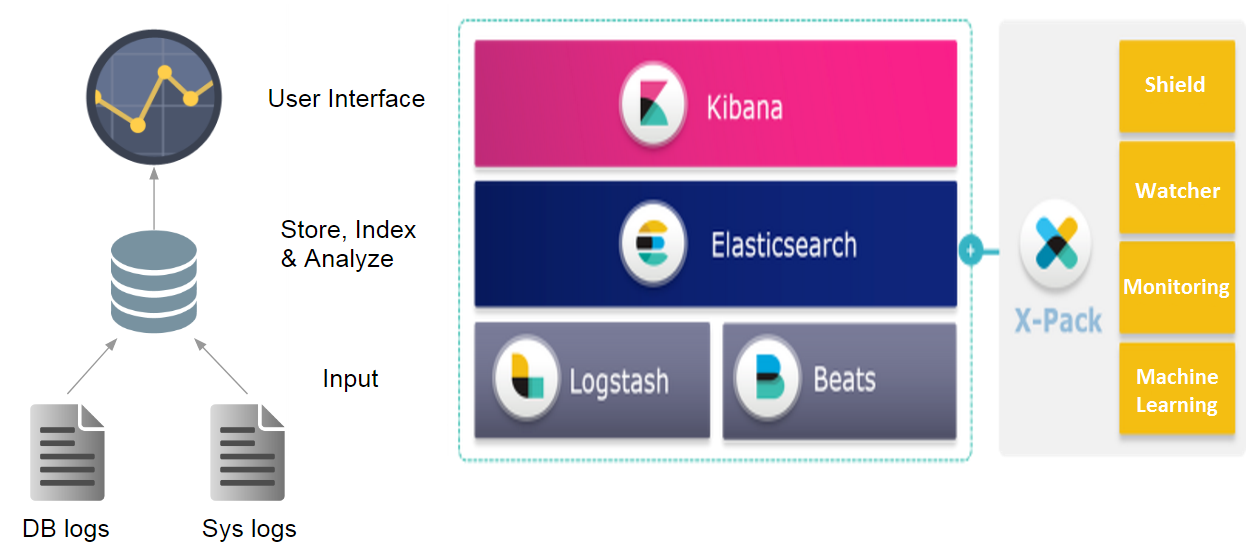
\includegraphics[width=16cm]{img/elasticstackoverview}
	\caption{Overzicht Elastic stack}
	\label{fig:elasticstackoverview}
\end{figure}

Zoals te zien is op in \ref{fig:elasticstackoverview} bestaat Elastic stack uit drie niveaus. 
Om de werking uit te leggen moet onderaan begonnen worden. Op dit niveau staan Logstash en Beats. 
Beats staat in voor het verzamelen van alle log files. Het is een tool die alle logs kan verzenden naar een centrale server waarop Logstash zich dan bevind. Logstash leest log files en verwerkt alle nieuwe lijnen die in de file geschreven worden. Het neemt lijn per lijn en verwerkt deze tot een json element.

Een niveau hoger is Elasticsearch te vinden. Elasticsearch staat in voor het opslaan en verwerken van alle input dat het krijgt van Logstash. Het krijgt de json elementen die logstash aanmaakt en slaat deze zo op in zijn databank. Doordat het json elementen zijn werkt de manier van zoeken op een andere dan met sql-opdrachten. In het verder verloop van deze bachelorproef zal gesproken over elementen dit zijn dan json elementen die zich in de database bevinden.

Kibana is de grafische kant van het hele gebeuren. Hier kan een overzicht van alle elementen getoond worden, het uitvoeren van Elasticsearch queries, het maken van grafieken, \dots.
Eenmaal alles geïmplementeerd is zal (in normale omstandigheden) alle acties via Kibana verlopen.

Helemaal rechts kan dan nog X-Pack gevonden worden. Dit is een samen raapsel van tools die werken met Elastic stack. 

%%=============================================================================
%% Conclusie
%%=============================================================================

\chapter{Conclusie}
\label{ch:conclusie}

Elastic stack voldoet aan alle vereisten vooropgesteld door oXya. Indien beslist zou worden om er mee verder te gaan zal een analyse gemaakt moeten worden van welke andere log files nog gebruikt kunnen worden. Voor deze files zal dan een logstash config file geschreven moeten worden. 
Dit zorgt er voor dat de implementatie wel wat werk zal vergen maar daarna werkt het volledig autonoom. Elastic stack zou er dan voor zorgen dat sommige problemen vroegtijdig gemeldt kunnen worden. Sommige tools en het dashboard kunnen dan geraadpleegd worden bij het onderzoeken van het probleem.

Naar de toekomst toe zijn dus heel wat mogelijkheden. Elastic stack is ook nog steeds erg snel aan het groeien en zal dus nog meer mogelijkheden bieden in de toekomst. Voor oXya is dit, volgens de geschetste casus, een gepast product. Maar de uitdaging zal liggen in het op de gepaste tijd zenden van meldingen.
Een mogelijk vervolg onderzoek zou kunnen zijn naar de anomaly detectie.
Een andere mogelijkheid zou zijn naar het zelf schrijven van elastic aangezien het open scource is en een java api heeft.

Hieronder wordt de mening van oXya zelf gegeven:


	``De eerste resultaten bij het gebruik van Elastic stack om een bijkomende vorm van monitoring te hebben, lijken zeer positief. 
	De mogelijkheid om verschillenden logfiles van uiteenlopende systemen (os, db , sap) te analyseren en daarin bepaalde kritische alerts te detecteren en te escaleren is zeer bruikbaar in onze omgeving. 
	Het online oppikken van alerts was een optie die te verwachten was van deze tool. 
	Maar wat nog interessanter blijkt te zijn, is het gedrag van bepaalde loglijnen in log-files te laten analyseren en te laten interpreteren met de “Timelion” en de “Machine Learning“ modules.
	Wat de mogelijkheid geeft om statische beslissingen te treffen, tijdens het analyseren van deze (soms seasonal) data. 
	Bijvoorbeeld het gebruik van de "Seasonal Holt-Winters" methode om abnormaal gedrag te voorspellen, lijken duidelijk een stap in de goede richting. 
	Waar we vroeger enkel triggers gebruikten om alerts te generen, kunnen we nu ook anomalieën vroegtijdig detecteren. 
	Gezien er nog veel mogelijkheden te onderzoeken zijn in het domein van machine learning zijn we zeker van plan nog verder onderzoek in te plannen op dit terrein.''
	\begin{flushright} 
		-Van Den Abeele, Martin
    \end{flushright}


%%---------- Back matter ------------------------------------------------------

\printbibliography
\addcontentsline{toc}{chapter}{\textcolor{maincolor}{\IfLanguageName{dutch}{Bibliografie}{Bibliography}}}


\listoffigures
\listoftables

\end{document}
